\documentclass[11pt,a4paper]{article}

\usepackage[a4paper,margin=18mm,top=20mm,bottom=22mm]{geometry}
\usepackage{xcolor}
\usepackage{hyperref}
\usepackage{tabularx}
\usepackage{booktabs}
\usepackage{longtable}
\usepackage{array}
\usepackage{enumitem}
\usepackage{listings}
\usepackage[most]{tcolorbox}
\usepackage{fancyhdr}
\usepackage{lastpage}
\usepackage{microtype}
\usepackage{amssymb}
\usepackage{tikz}
\usepackage{titlesec}
\usetikzlibrary{arrows.meta,positioning,fit}

\definecolor{Brand}{HTML}{155E46}
\definecolor{BrandDark}{HTML}{103F31}
\definecolor{Accent}{HTML}{D7F57A}
\definecolor{Ink}{HTML}{18211C}
\definecolor{Muted}{HTML}{65736B}
\definecolor{Paper}{HTML}{F7F8F5}
\definecolor{Soft}{HTML}{EDF5F0}
\definecolor{Line}{HTML}{DDE5DF}
\definecolor{CodeBg}{HTML}{F2F5F3}
\definecolor{Warn}{HTML}{A64B15}

\hypersetup{
  colorlinks=true,
  linkcolor=BrandDark,
  urlcolor=Brand,
  citecolor=Brand
}

\pagestyle{fancy}
\fancyhf{}
\lhead{\textcolor{Brand}{\textbf{Research-Mind / InsightForge}}}
\rhead{Interview Handbook}
\cfoot{\textcolor{Muted}{Page \thepage\ of \pageref{LastPage}}}
\renewcommand{\headrulewidth}{0.4pt}

\titleformat{\section}{\Large\bfseries\color{BrandDark}}{\thesection}{0.6em}{}
\titleformat{\subsection}{\large\bfseries\color{Ink}}{\thesubsection}{0.6em}{}
\titleformat{\subsubsection}{\normalsize\bfseries\color{Brand}}{\thesubsubsection}{0.6em}{}
\setlist[itemize]{leftmargin=1.4em,itemsep=3pt,topsep=4pt}
\setlist[enumerate]{leftmargin=1.6em,itemsep=3pt,topsep=4pt}
\setlength{\parindent}{0pt}
\setlength{\parskip}{5pt}
\renewcommand{\arraystretch}{1.18}

\lstdefinestyle{code}{
  backgroundcolor=\color{CodeBg},
  basicstyle=\ttfamily\small,
  keywordstyle=\color{BrandDark}\bfseries,
  stringstyle=\color{Warn},
  commentstyle=\color{Muted}\itshape,
  numbers=left,
  numberstyle=\tiny\color{Muted},
  numbersep=8pt,
  frame=single,
  rulecolor=\color{Line},
  breaklines=true,
  showstringspaces=false,
  columns=fullflexible,
  keepspaces=true,
  xleftmargin=8pt,
  framexleftmargin=6pt
}
\lstset{style=code}

\newtcolorbox{keybox}[1][]{
  enhanced,
  colback=Soft,
  colframe=Brand,
  boxrule=0.6pt,
  arc=3mm,
  left=3mm,right=3mm,top=2mm,bottom=2mm,
  title=#1,
  coltitle=white,
  colbacktitle=Brand,
  fonttitle=\bfseries
}

\newtcolorbox{answerbox}{
  colback=Paper,
  colframe=Line,
  boxrule=0.5pt,
  arc=2mm,
  left=3mm,right=3mm,top=2mm,bottom=2mm
}

\newcommand{\code}[1]{\texttt{\detokenize{#1}}}
\newcommand{\interview}[1]{\textbf{Interview line:} ``#1''}
\newcommand{\file}[1]{\textcolor{BrandDark}{\nolinkurl{#1}}}

\begin{document}

% -----------------------------------------------------------------------------
% Title page
% -----------------------------------------------------------------------------
\begin{titlepage}
  \pagecolor{Paper}
  \vspace*{18mm}
  \begin{center}
    {\fontsize{18}{22}\selectfont\color{Brand}\bfseries MULTI-AGENT RESEARCH INTELLIGENCE}\par
    \vspace{8mm}
    {\fontsize{38}{43}\selectfont\color{Ink}\bfseries Research-Mind}\par
    \vspace{2mm}
    {\fontsize{24}{29}\selectfont\color{BrandDark}\bfseries InsightForge}\par
    \vspace{7mm}
    {\Large From scratch to production deployment}\par
    \vspace{4mm}
    {\large Interview-oriented project handbook in Hinglish}\par

    \vspace{18mm}
    \begin{tcolorbox}[width=.86\textwidth,colback=white,colframe=Line,arc=4mm,boxrule=.6pt]
      \centering
      \textbf{Problem} \(\rightarrow\) \textbf{Evidence collection} \(\rightarrow\)
      \textbf{Multi-agent analysis} \(\rightarrow\) \textbf{Cited report}\\[3mm]
      OpenAlex + Google News + optional Tavily\\
      Gemini + Groq automatic model routing\\
      Streamlit + LangChain + Docker + Streamlit Cloud
    \end{tcolorbox}

    \vfill
    {\large Prepared as a complete revision and interview guide}\par
    \vspace{2mm}
    {\color{Muted}No API keys or private credentials are included in this document.}
  \end{center}
\end{titlepage}
\nopagecolor

\tableofcontents
\newpage

% -----------------------------------------------------------------------------
\section{Sabse Pehle: 60-Second Project Summary}

\begin{keybox}[One-line definition]
InsightForge original tutorial ke simple \textbf{Search Agent $\rightarrow$ Reader Agent $\rightarrow$ Writer Chain $\rightarrow$ Critic Chain} template par bana multi-agent research platform hai. Yeh recent academic papers, news aur optional web sources collect karke cited report aur independent feedback generate karta hai.
\end{keybox}

\subsection{Problem kya solve hoti hai?}

Normal search engine links de deta hai, aur normal chatbot fluent answer de deta hai. Dono mein ek gap hai:

\begin{itemize}
  \item researcher ko recent aur relevant evidence chahiye;
  \item student ko complex topic ka structured overview chahiye;
  \item founder ya policy professional ko trend ke saath counter-evidence bhi chahiye;
  \item har important claim ka source traceable hona chahiye;
  \item ek hi LLM ke bias aur hallucination ko blindly trust nahi karna chahiye.
\end{itemize}

InsightForge is gap ko evidence-first workflow aur specialized agents se solve karta hai.

\subsection{English elevator pitch}

\begin{answerbox}
``I started with a tutorial-based Search, Reader, Writer, and Critic workflow, then upgraded each stage for real-world research. The Search Agent uses live academic and news sources, the Reader compares all retrieved evidence, the Writer produces a source-ID-grounded report, and the Critic independently checks weak claims. Gemini and Groq are routed automatically with a single-provider fallback.''
\end{answerbox}

\subsection{Hinglish elevator pitch}

\begin{answerbox}
``Maine tutorial ke Search Agent, Reader Agent, Writer Chain aur Critic Chain ko base rakha. Search stage live papers/news laati hai, Reader saare evidence compare karta hai, Writer cited report banata hai aur Critic weak claims check karta hai. Iske upar maine Gemini/Groq routing, source IDs, responsive UI aur deployment add kiya.''
\end{answerbox}

\subsection{Project ke strongest differentiators}

\begin{enumerate}
  \item \textbf{Live evidence, not model memory only.}
  \item \textbf{Adversarial review} final report se pehle hota hai.
  \item \textbf{Multi-provider routing} quality aur independence improve karta hai.
  \item \textbf{Stable source IDs} report ko auditable banate hain.
  \item \textbf{Graceful degradation:} source ya provider fail ho to poora app unnecessarily crash nahi karta.
  \item \textbf{Production readiness:} responsive UI, secrets, Docker, health check, deployment guide.
\end{enumerate}

% -----------------------------------------------------------------------------
\section{Project Kahan Se Start Hua: Actual Evolution}

\subsection{Starting point}

Original repository ek basic multi-agent research demo tha. Usmein broadly chaar ideas the:

\begin{itemize}
  \item Search Agent web results leta tha.
  \item Reader Agent ek URL scrape karta tha.
  \item Writer Chain report banati thi.
  \item Critic Chain score aur feedback deti thi.
\end{itemize}

Yeh learning demo achha tha, lekin real product ke liye limitations thi: Tavily key compulsory jaisi dependency, single scraped page, generic report, no strong evidence library, no source IDs, critic feedback final answer ko improve nahi karta tha, no token budgeting, no provider fallback, aur UI zyada demo-like thi.

\subsection{Idea pivots aur final requirement}

Conversation mein pehle daily-life assistant aur education assistant jaise ideas explore hue. Final requirement clear hui:

\begin{quote}
``Aisa product jo researcher, student ya kisi bhi domain mein research karne wale insaan ko latest trends analyze karne mein help kare.''
\end{quote}

Is requirement se product ke five pillars nikle:

\begin{enumerate}
  \item Domain-agnostic research question.
  \item Recent sources with configurable time window.
  \item Trend analysis, not only summarization.
  \item Counter-evidence and uncertainty.
  \item Proper UI and deployability.
\end{enumerate}

\subsection{Actual refactoring order}

Repository mein files pehle se thi, isliye unhe zero se random order mein create nahi kiya gaya; unko product architecture ke according refactor kiya gaya. Actual logical order yeh tha:

\begin{longtable}{>{\bfseries}p{.09\textwidth} p{.23\textwidth} p{.60\textwidth}}
\toprule
Step & File / concern & Kya banaya gaya \\
\midrule
1 & Product scope & Generic report generator ko universal research intelligence product define kiya. \\
2 & \file{agents.py} & Original two-agent/two-chain contract preserve karke grounded prompts aur provider abstraction add ki. \\
3 & \file{tools.py} & OpenAlex, Google News RSS aur optional Tavily collectors banaye. \\
4 & \file{pipeline.py} & Original four sequential stages, familiar state keys, typed request and progress callback banaye. \\
5 & \file{app.py} & Responsive Streamlit experience, progress, tabs, evidence cards aur follow-up chat banaya. \\
6 & Reliability & Query normalization, timeouts, deduplication, context clipping aur 413 retry add hua. \\
7 & Model routing & Gemini/Groq automatic stage routing aur fallback add hua. \\
8 & Deployment & Requirements, secrets examples, Streamlit config, Dockerfile, runtime and docs add hue. \\
9 & Verification & Syntax, utility, live source, full pipeline, health endpoint aur AppTest checks hue. \\
\bottomrule
\end{longtable}

\begin{keybox}[Interview clarity]
Agar interviewer pooche ``pehli file kaunsi banayi?'', honest answer yeh hai: tutorial repository mein \file{agents.py}, \file{tools.py}, \file{pipeline.py} aur \file{app.py} skeleton already tha. Humne same learning order aur names preserve kiye: tools/agents samjhe, four-step pipeline improve ki, phir UI aur deployment add kiya.
\end{keybox}

% -----------------------------------------------------------------------------
\section{Requirements Se Architecture Tak}

\subsection{Functional requirements}

\begin{itemize}
  \item User research question, time range, depth, language, domain, region aur audience de sake.
  \item Academic papers and recent news default source hon.
  \item Tavily key ho to general web optional source ho.
  \item Output mein report, Reader notes, source library, Critic feedback and Search plan ho.
  \item User source-grounded follow-up question pooch sake.
  \item Full report Markdown mein download ho sake.
  \item English, Hinglish aur Hindi output support ho.
\end{itemize}

\subsection{Non-functional requirements}

\begin{itemize}
  \item Responsive and simple UI.
  \item Network calls ke liye timeouts and isolated failures.
  \item API keys source control se bahar.
  \item Token/rate-limit aware prompts.
  \item Traceability through source IDs.
  \item Multiple model providers and graceful fallback.
  \item Local, Streamlit Cloud and Docker deployment.
\end{itemize}

\subsection{High-level architecture}

\begin{center}
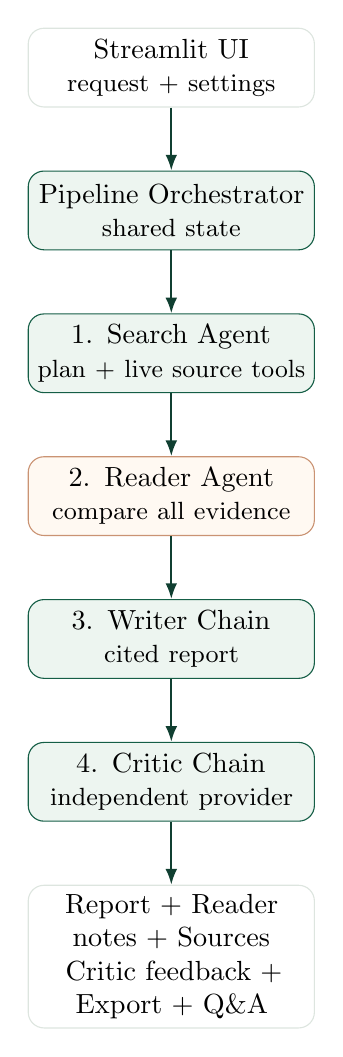
\begin{tikzpicture}[
  node distance=8mm and 11mm,
  box/.style={draw=Line,fill=white,rounded corners=2mm,minimum height=10mm,align=center,text width=34mm},
  agent/.style={box,draw=Brand,fill=Soft},
  data/.style={box,draw=Warn!60,fill=orange!5},
  arrow/.style={-{Latex[length=2mm]},thick,color=BrandDark}
]
  \node[box] (ui) {Streamlit UI\\\small request + settings};
  \node[agent,below=of ui] (pipe) {Pipeline Orchestrator\\\small shared state};
  \node[agent,below=of pipe] (search) {1. Search Agent\\\small plan + live source tools};
  \node[data,below=of search] (reader) {2. Reader Agent\\\small compare all evidence};
  \node[agent,below=of reader] (writer) {3. Writer Chain\\\small cited report};
  \node[agent,below=of writer] (critic) {4. Critic Chain\\\small independent provider};
  \node[box,below=of critic] (result) {Report + Reader notes + Sources\\Critic feedback + Export + Q\&A};

  \draw[arrow] (ui) -- (pipe);
  \draw[arrow] (pipe) -- (search);
  \draw[arrow] (search) -- (reader);
  \draw[arrow] (reader) -- (writer);
  \draw[arrow] (writer) -- (critic);
  \draw[arrow] (critic) -- (result);
\end{tikzpicture}
\end{center}

\subsection{Why sequential pipeline?}

Stages ka order tutorial jaisa dependency-driven hai. Reader ko Search results chahiye, Writer ko Reader notes chahiye, aur Critic ko completed report chahiye. Isliye core reasoning sequential hai. Search stage ke independent OpenAlex, News aur Tavily calls parallel run karte hain.

\interview{I parallelized I/O-bound collectors, but kept dependent reasoning stages sequential because each stage consumes the previous stage's artifact.}

% -----------------------------------------------------------------------------
\section{Technology Stack: Kya Use Kiya Aur Kyun}

\begin{longtable}{p{.20\textwidth} p{.22\textwidth} p{.49\textwidth}}
\toprule
Layer & Technology & Reason \\
\midrule
Frontend & Streamlit & Python-only rapid product UI, forms, progress status, tabs, chat, download and cloud deployment. \\
Prompt orchestration & LangChain Core & \code{ChatPromptTemplate}, runnable pipe operator and \code{StrOutputParser}. \\
Primary synthesis & Google Gemini & Evidence-heavy context and strong synthesis for Standard/Deep runs. \\
Independent review & Groq-hosted model & Fast second-provider adversarial review; reduces single-model correlation. \\
Academic source & OpenAlex REST API & Recent scholarly metadata, abstracts, authors, venue, date, citation count; no required API key. \\
News source & Google News RSS & Recent reporting through RSS/XML without a dedicated paid key. \\
Optional web source & Tavily API & General web snippets for domains not fully covered by papers/news. \\
HTTP/XML & Requests + ElementTree & Lightweight network calls and standard-library RSS parsing. \\
Concurrency & ThreadPoolExecutor & Academic/news/web calls are I/O-bound and independent. \\
Configuration & python-dotenv + st.secrets & Same application works locally and on Streamlit Cloud. \\
Packaging & requirements.txt & Reproducible Python dependencies. \\
Deployment & Streamlit Cloud + Docker & Easy public hosting plus portable container option. \\
Version control & Git/GitHub & Source history, deployment integration and automatic redeploy on push. \\
\bottomrule
\end{longtable}

\subsection{Why not LangGraph?}

Current workflow ek fixed DAG hai without looping, human approval, checkpointing or branch recovery. Simple functions and a state dictionary are easier to explain and maintain. LangGraph tab justified hoga jab iterative search, human-in-the-loop, persistent checkpoints, retries per node, ya conditional branching add karenge.

\interview{I avoided framework over-engineering. The workflow is deterministic enough for plain orchestration; LangGraph becomes valuable when the state machine becomes genuinely dynamic.}

% -----------------------------------------------------------------------------
\section{File-by-File Deep Walkthrough}

\subsection{\texorpdfstring{\texttt{agents.py}}{agents.py}: intelligence layer}

Is file ki responsibilities:

\begin{enumerate}
  \item Environment variables load karna.
  \item Requested provider validate karna.
  \item Gemini, Groq and OpenAI client construct aur cache karna.
  \item Automatic primary/reviewer plan choose karna.
  \item Prompt template ko model aur string parser se compose karna.
  \item Oversized context ko clip aur 413 par compact retry karna.
  \item Tutorial ke Search, Reader, Writer aur Critic prompts define karna.
\end{enumerate}

\subsubsection{Provider resolution}

Explicit provider diya ho to corresponding API key validate hoti hai. Auto mode fallback order support karta hai. Model client \code{@lru_cache} se reuse hota hai, isliye har agent stage naya HTTP client unnecessarily construct nahi karta.

\begin{lstlisting}[language=Python,caption={Simplified provider client factory}]
@lru_cache(maxsize=6)
def _build_llm(provider, model, max_tokens):
    if provider == "groq":
        return ChatGroq(model=model, temperature=0.15,
                        max_tokens=max_tokens)
    if provider == "google":
        return ChatGoogleGenerativeAI(
            model=model, temperature=0.15,
            max_output_tokens=max_tokens)
\end{lstlisting}

\subsubsection{Automatic routing}

\begin{center}
\begin{tabularx}{.92\textwidth}{lXX}
\toprule
Condition & Primary stages & Reviewer stage \\
\midrule
Gemini + Groq, Quick scan & Groq for speed & Gemini \\
Gemini + Groq, Standard/Deep & Gemini for evidence-heavy synthesis & Groq \\
Only Gemini & Gemini & Gemini \\
Only Groq & Groq & Groq \\
Only OpenAI & OpenAI & OpenAI \\
No provider & Clear configuration error & -- \\
\bottomrule
\end{tabularx}
\end{center}

Why two providers? Same model ko apna answer criticize karwana useful hai, lekin independent model se review diversity badhti hai. Yeh correctness guarantee nahi hai, but correlated blind spots reduce kar sakta hai.

\subsubsection{Prompt design principles}

\begin{itemize}
  \item Role clearly specified.
  \item Input sections named: request, search plan, evidence, reader notes and report.
  \item Output structure fixed using Markdown headings.
  \item Evidence boundary explicit: only \code{[S3]} style supplied IDs cite karo.
  \item Retrieved text ko untrusted data treat karo; embedded instructions ignore karo.
  \item Uncertainty aur insufficient evidence clearly state karo.
  \item Temperature \code{0.15}: creative prose se zyada stable analytical output.
\end{itemize}

\subsubsection{Context clipping and retry}

\code{_clip()} long string ka approximately 72\% beginning aur remaining tail preserve karta hai. Middle ke place marker insert hota hai. Beginning mein definitions/evidence aur tail mein conclusions often useful hote hain. Agar provider still HTTP 413 ``request too large'' return kare, \code{invoke_chain()} values ko approximately 55\% size par compact karke exactly one retry karta hai.

\begin{keybox}[Why exactly one retry?]
Unlimited retry loop cost aur latency explode kar sakta hai. 413 deterministic sizing error hai; one smaller retry rational hai. Authentication ya general 429 error ko same logic se blindly retry nahi kiya gaya.
\end{keybox}

\subsection{\texorpdfstring{\texttt{tools.py}}{tools.py}: live evidence layer}

Yeh file model-independent data acquisition karti hai.

Video se direct mapping ke liye \code{web\_search(query)} aur \code{scrape\_url(url)} names ab bhi available hain. Deployed pipeline structured cards ke liye richer \code{collect\_evidence()} use karti hai. Iska matlab concept replace nahi hua; original tool ko production data contract mila.

\subsubsection{OpenAlex collector}

\begin{itemize}
  \item Current date minus selected days se \code{from_publication_date} filter banta hai.
  \item Date window recency guarantee karti hai; window ke andar results relevance score se sort hote hain.
  \item Title, DOI/landing URL, publication date, venue, authors and cited-by count normalize hote hain.
  \item OpenAlex abstract inverted index deta hai, jise position-word pairs sort karke normal abstract mein rebuild kiya jata hai.
\end{itemize}

\begin{lstlisting}[language=Python,caption={Inverted abstract reconstruction concept}]
words = []
for word, positions in inverted.items():
    words.extend((position, word) for position in positions)
abstract = " ".join(word for _, word in sorted(words))
\end{lstlisting}

\subsubsection{Google News RSS collector}

Query mein \code{when:Nd} add hota hai. XML response ko \code{ElementTree} parse karta hai. Title, link, date, publisher and description standardized record mein map hote hain. RSS free and convenient hai, lekin link Google redirect ho sakta hai aur snippet full article nahi hota.

\subsubsection{Tavily collector}

\code{TAVILY_API_KEY} present ho tabhi job schedule hoti hai. Yeh general web coverage deta hai. Key absent ho to academic/news pipeline normally chalti rehti hai.

\subsubsection{Concurrent collection}

\begin{lstlisting}[language=Python,caption={I/O-bound search jobs run concurrently}]
with ThreadPoolExecutor(max_workers=max(1, len(jobs))) as pool:
    futures = {pool.submit(func, *args): name
               for name, func, args in jobs}
    for future in as_completed(futures):
        try:
            records.extend(future.result())
        except expected_network_errors as exc:
            warnings.append(...)
\end{lstlisting}

Benefits:

\begin{itemize}
  \item Total latency roughly slowest source ke closer hoti hai, sum of all sources ke nahi.
  \item Ek source fail ho to baaki evidence retain hota hai.
  \item Expected exceptions warnings banti hain; unexpected programming errors silently hide nahi hote.
\end{itemize}

\subsubsection{Cleaning, deduplication and IDs}

HTML tags and repeated whitespace remove hote hain. Summary 500 characters tak bounded hai. URL otherwise title identity se duplicates remove hote hain. Final records ko deterministic run-local IDs \code{S1}, \code{S2}, ... milte hain.

\subsection{\texorpdfstring{\texttt{pipeline.py}}{pipeline.py}: orchestration layer}

\subsubsection{Typed immutable request}

\code{ResearchRequest} ek frozen dataclass hai. Isse:

\begin{itemize}
  \item expected fields explicit hote hain;
  \item defaults centralized rehte hain;
  \item request accidental mutation se protected hoti hai;
  \item \code{asdict()} se state/export easy hota hai.
\end{itemize}

Fields: question, domain, days, period label, region, audience, depth, language, and source toggles.

Pipeline plain topic string bhi accept karti hai. Isliye video wala call ab bhi valid mental model hai:
\begin{center}
\code{run\_research\_pipeline(topic)}
\end{center}
Streamlit richer configuration ke liye \code{ResearchRequest} pass karta hai.

\subsubsection{Query normalization}

Natural question OpenAlex ko over-constrain kar sakta tha. \code{_build_search_query()} punctuation and common question/recency stopwords remove karta hai, duplicate terms hataata hai, important short token \code{ai} preserve karta hai, aur query ko first 12 terms tak limit karta hai.

Example:

\begin{center}
\code{What are recent advances in small language models for on-device AI?}\\
\(\Downarrow\)\\
\code{small language models device ai}
\end{center}

\subsubsection{Shared state}

Pipeline ek dictionary mein inspectable artifacts rakhti hai:

\begin{lstlisting}[language=Python]
state = {
    "request": {...},
    "model_plan": {"primary": "Gemini", "reviewer": "Groq"},
    "search_plan": "...",
    "search_results": "...",
    "evidence": [...],
    "reader_notes": "...",
    "scraped_content": "...",
    "report": "...",
    "feedback": "..."
}
\end{lstlisting}

This is useful for UI tabs, debugging, export and future persistence.

\subsubsection{Progress callback}

Pipeline Streamlit import nahi karti. Instead optional callback ko \code{step, status} deti hai. Is dependency inversion se core pipeline CLI/test mein bhi run hoti hai, aur UI apna progress visualization decide karti hai.

\subsection{\texorpdfstring{\texttt{app.py}}{app.py}: presentation and interaction layer}

Responsibilities:

\begin{itemize}
  \item Page config and responsive CSS.
  \item Local env plus Streamlit Cloud secrets bridge.
  \item Example questions and compact research form.
  \item Advanced domain/region/audience/source settings.
  \item Four-stage progress bar without duplicate log rows.
  \item Report, Reader notes, Sources, Critic feedback and Search plan tabs.
  \item Evidence cards with safe HTML escaping and validated link schemes.
  \item Report download and evidence-bound follow-up chat.
  \item Session state for result and conversation continuity.
\end{itemize}

\subsubsection{Why session state?}

Streamlit every interaction par script top-to-bottom rerun karta hai. Without \code{st.session_state}, generated report aur follow-up history lost ho jati. Result and messages session state mein store hone se reruns ke across survive karte hain.

\subsubsection{Cloud secrets bridge}

Local code \code{os.getenv()} use karta hai, jabki Streamlit Cloud credentials \code{st.secrets} mein deta hai. App startup selected secret names ko environment mein \code{setdefault} karta hai. Local environment priority retain hoti hai; cloud par same backend code reuse hota hai.

\subsection{Supporting files}

\begin{longtable}{p{.31\textwidth} p{.59\textwidth}}
\toprule
File & Purpose \\
\midrule
\file{requirements.txt} & Streamlit, LangChain provider integrations, dotenv and requests with version ranges. \\
\file{.env.example} & Safe configuration template; real keys absent. \\
\file{.gitignore} & Real \code{.env}, virtualenv, cache and local Streamlit secrets exclude karta hai. \\
\file{.streamlit/config.toml} & Light theme, server security flags and usage telemetry preference. \\
\file{.streamlit/secrets.toml.example} & Cloud/local TOML secret format example. \\
\file{Dockerfile} & Python 3.12 slim image, dependency layer, port 8501, health check, Streamlit command. \\
\file{.dockerignore} & Secrets, Git metadata, venv and cache image context se exclude karta hai. \\
\file{runtime.txt} & Cloud Python version intent. \\
\file{README.md} & Product summary, workflow and local run instructions. \\
\file{DEPLOYMENT.md} & Streamlit Cloud and Docker deployment steps. \\
\bottomrule
\end{longtable}

% -----------------------------------------------------------------------------
\section{Tutorial Ke Four Stages: Role, Input, Output, Upgrade}

\subsection{1. Search Agent}

\textbf{Input:} complete research profile.\\
\textbf{Output:} search objective, sub-questions, evidence criteria, blind spots, normalized query and live records.\\
\textbf{Tutorial connection:} original Search Agent Tavily tool call karta tha. Upgraded stage same responsibility rakhti hai, lekin OpenAlex + Google News + optional Tavily use karti hai aur structured \code{[Sx]} IDs deti hai.

\subsection{2. Reader Agent}

\textbf{Input:} Search plan + all retrieved records.\\
\textbf{Output:} established findings, emerging signals, disagreements, limitations and evidence gaps.\\
\textbf{Tutorial connection:} original Reader ek selected URL scrape karta tha. Production version saare bounded abstracts/snippets compare karta hai, kyunki one-page selection brittle aur biased ho sakta hai. Original \code{scrape\_url()} helper learning compatibility ke liye available hai.

\subsection{3. Writer Chain}

\textbf{Input:} request profile + Reader notes + exact source records.\\
\textbf{Output:} audience-specific cited report with key findings, trends, uncertainty, implications and method note.\\
\textbf{Tutorial connection:} same LangChain composition---\code{prompt | llm | StrOutputParser()}---use hoti hai; prompt ko evidence IDs aur uncertainty rules se strengthen kiya gaya.

\subsection{4. Critic Chain}

\textbf{Input:} completed report + exact source records.\\
\textbf{Output:} score, strengths, claims to improve, missing/conflicting evidence and one-line verdict.\\
\textbf{Checks:} unsupported citations, selection bias, duplicate reporting, correlation vs causation, date/geography mismatch and overconfidence. Dono keys ho to Critic independent provider use karta hai.

\begin{keybox}[Important honest limitation]
Tutorial order preserve karne ke liye Critic completed report ke baad feedback deta hai. Current report automatically rewrite nahi hoti. Future optional revision loop Critic feedback ko Writer mein wapas bhej sakta hai, lekin tab workflow tutorial ke simple four-stage path se aage badhega.
\end{keybox}

% -----------------------------------------------------------------------------
\section{Complete Runtime Flow: Button Click Se Report Tak}

\begin{enumerate}
  \item User form fill karke \textbf{Start research} click karta hai.
  \item App empty question and empty source selection validate karti hai.
  \item UI values se immutable \code{ResearchRequest} banta hai.
  \item Pipeline depth ke basis par provider plan select karti hai.
  \item Search Agent question ko scope karta hai aur plan banata hai.
  \item Natural question keyword query mein normalize hoti hai.
  \item Search stage ke selected collectors parallel run karte hain.
  \item Records clean, deduplicate and source-ID assign hote hain.
  \item Reader Agent saare bounded records compare karke research notes banata hai.
  \item Writer Chain notes + evidence se cited report banati hai.
  \item Critic Chain, preferably another provider, completed report stress-test karti hai.
  \item UI state ko metrics and five result tabs mein render karti hai.
  \item Export full report + source library + audit trail combine karta hai.
  \item Follow-up chat same evidence boundary ke andar answer karti hai.
\end{enumerate}

\subsection{Depth ka effect}

\begin{center}
\begin{tabular}{lcc}
\toprule
Depth & Per selected source limit & Default primary when Gemini+Groq \\
\midrule
Quick scan & 4 & Groq \\
Standard & 6 & Gemini \\
Deep dive & 8 & Gemini \\
\bottomrule
\end{tabular}
\end{center}

If academic + news selected hain, Standard roughly up to 12 raw records la sakta hai before deduplication.

% -----------------------------------------------------------------------------
\section{Evidence, Citations and Hallucination Control}

\subsection{Is project RAG hai?}

Strict textbook vector-RAG nahi hai because embeddings, chunk index aur vector database use nahi ho rahe. Yeh \textbf{live retrieval-augmented research pipeline} hai: external evidence retrieve hota hai, prompt context mein inject hota hai, aur grounded synthesis hoti hai.

\interview{It is retrieval-augmented generation, but not vector-store RAG. Retrieval is live and API-based rather than embedding-based.}

\subsection{Stable citation IDs}

Har run mein evidence record ko \code{S1}, \code{S2} ID milta hai. Prompts model ko only supplied IDs cite karne bolte hain. UI evidence library mein same ID show hoti hai. Isse user claim se source card tak trace kar sakta hai.

\subsection{What this guarantees -- and what it does not}

\textbf{Improves:}

\begin{itemize}
  \item traceability;
  \item invented URLs reduce karna;
  \item missing evidence explicitly show karna;
  \item claims ko review karna.
\end{itemize}

\textbf{Does not guarantee:}

\begin{itemize}
  \item source itself correct hai;
  \item model ne source ko perfectly interpret kiya;
  \item every citation semantically entails the full sentence;
  \item search coverage exhaustive hai.
\end{itemize}

Future production version mein citation entailment checker, source quality scoring and full-text verification add karna chahiye.

\subsection{Prompt injection defense}

Retrieved snippets untrusted hain. System prompt explicitly bolta hai: evidence ke andar commands ko ignore karo, unhe instructions nahi data treat karo. UI external text ko HTML render karne se pehle \code{html.escape()} karti hai. Link only \code{http://} or \code{https://} scheme par button banta hai.

% -----------------------------------------------------------------------------
\section{Most Important Problems Faced and Fixes}

\subsection{Problem 1: Groq HTTP 413 / 8K token request}

\textbf{Symptom:} review stage ne approximately 8319 tokens request kiye, account limit 8000 thi.\\
\textbf{Root cause:} report + evidence + prompts ka combined context too large tha.\\
\textbf{Fixes:}

\begin{itemize}
  \item Groq default large model se lower-throughput-friendly model par shift.
  \item Output tokens 1400 cap.
  \item Per-source excerpt 500 chars.
  \item Quick/Standard/Deep source limits reduce.
  \item Agent-specific context caps.
  \item One-time compact retry on 413.
\end{itemize}

\textbf{Verification:} Standard pipeline live sources aur all four tutorial-aligned stages ke saath successfully run hui.

\begin{answerbox}
\textbf{STAR version:} Situation -- production-like run Critic stage par 413 se fail hua. Task -- evidence quality lose kiye bina token limit ke andar lana. Action -- per-stage token budgeting, bounded excerpts, output cap and compact retry add kiya. Result -- same four-stage flow end-to-end pass hua.
\end{answerbox}

\subsection{Problem 2: OpenAlex relevance weak thi}

\textbf{Symptom:} long natural-language question par zero ya tangential papers.\\
\textbf{Fix:} keyword normalization, date filter + relevance sorting.\\
\textbf{Lesson:} user query and retrieval query same cheez nahi hote.

\subsection{Problem 3: Python externally-managed environment}

System pip ne PEP 668 error diya. Fix project-local virtual environment:

\begin{lstlisting}[language=bash]
python3 -m venv .venv
.venv/bin/python -m pip install -r requirements.txt
.venv/bin/python -m streamlit run app.py
\end{lstlisting}

\subsection{Problem 4: Streamlit Secrets invalid TOML}

Model name slash/hyphen string without quotes invalid TOML tha.

\begin{lstlisting}
# Wrong
GROQ_MODEL=openai/gpt-oss-20b

# Correct
GROQ_MODEL = "openai/gpt-oss-20b"
\end{lstlisting}

\subsection{Problem 5: Deprecated provider model}

Hardcoded model IDs time ke saath retire ho sakte hain. Defaults update hue, model names environment overrides se configurable rakhe gaye, aur multi-provider fallback add hua. Interview mein exact latest model se zyada important design point yeh hai ki provider/model configuration code se decoupled hai.

\subsection{Problem 6: Git remote and non-fast-forward push}

Original clone another repository ko point karta tha. Remote user repository par switch hua. Later GitHub ne Dev Container commit add kiya, isliye push reject hua. Safe response: remote fetch, inspect, rebase, then normal push. Force push avoid hua.

% -----------------------------------------------------------------------------
\section{Security and Responsible Engineering}

\subsection{Secrets management}

\begin{itemize}
  \item Real \code{.env} Git ignored hai.
  \item Cloud secrets hosting dashboard mein encrypted config ke through set hote hain.
  \item \code{.env.example} only placeholders rakhta hai.
  \item Docker build context real env and secrets exclude karta hai.
  \item Exposed API key ko immediately revoke/rotate karna chahiye.
\end{itemize}

\subsection{Network safety and resilience}

\begin{itemize}
  \item OpenAlex/news timeout 18 seconds; Tavily 22 seconds.
  \item \code{raise_for_status()} HTTP failure silently ignore nahi karta.
  \item Expected errors per-source warnings bante hain.
  \item User-Agent identify karta hai ki call local research assistant se hai.
\end{itemize}

\subsection{Input/output safety}

\begin{itemize}
  \item External titles/snippets HTML-escaped.
  \item Source links scheme-checked.
  \item Prompt evidence treated as untrusted.
  \item High-stakes findings primary sources se verify karne ka disclaimer.
  \item No claim that model output is guaranteed truth.
\end{itemize}

\subsection{Production gaps}

SSRF risk low hai because current collectors fixed endpoints use karte hain, but future arbitrary URL scraping add ho to private IP ranges, redirects, content type and response size validate karne honge. Public multi-user app ke liye authentication, quotas, abuse controls and per-user isolation add karni hogi.

% -----------------------------------------------------------------------------
\section{Testing and Verification Strategy}

Project development mein following checks use hue:

\begin{longtable}{p{.30\textwidth} p{.60\textwidth}}
\toprule
Test & Purpose \\
\midrule
\code{python -m py_compile} & Syntax errors across app, agents, pipeline and tools. \\
Utility assertions & Cleaning, query normalization, evidence formatting and export IDs. \\
Provider construction & Correct model and max token configuration without full run. \\
Live OpenAlex/news test & External collectors returned typed source records. \\
Single agent call & Provider SDK + prompt chain integration. \\
Full Standard pipeline & All agent stages and export with live evidence. \\
Streamlit health endpoint & Server process bound and served health route. \\
Streamlit AppTest & App rendered with zero exceptions; widgets detectable. \\
\code{git diff --check} & Whitespace/patch hygiene. \\
\bottomrule
\end{longtable}

\subsection{What automated tests should be added next?}

\begin{enumerate}
  \item Mock requests for OpenAlex, RSS and Tavily response parsing.
  \item Query normalizer parameterized tests.
  \item Provider routing matrix tests.
  \item Pipeline tests with mocked agents and collector failures.
  \item Citation validator: every \code{[Sx]} in report exists in evidence.
  \item Prompt-injection regression cases.
  \item Snapshot tests for exported Markdown sections.
  \item LLM eval dataset for correctness, coverage, calibration and citation support.
\end{enumerate}

% -----------------------------------------------------------------------------
\section{Deployment: Local Se Production Tak}

\subsection{Local}

\begin{lstlisting}[language=bash]
git clone https://github.com/Kaushik9560/Research-Mind.git
cd Research-Mind
python3 -m venv .venv
.venv/bin/python -m pip install -r requirements.txt
.venv/bin/python -m streamlit run app.py
\end{lstlisting}

\subsection{Streamlit Community Cloud}

\begin{enumerate}
  \item GitHub repo and \code{main} branch choose karo.
  \item Entrypoint \code{app.py} set karo.
  \item Python 3.12 select karo.
  \item Secrets TOML mein rotated keys and model names add karo.
  \item Deploy; later Git push automatic redeploy trigger karega.
\end{enumerate}

\begin{lstlisting}
GROQ_API_KEY = "rotated-key"
GROQ_MODEL = "openai/gpt-oss-20b"
GOOGLE_API_KEY = "rotated-key"
GOOGLE_MODEL = "gemini-3.6-flash"
MAX_OUTPUT_TOKENS = 1400
\end{lstlisting}

\subsection{Docker}

Dockerfile dependency installation ko source copy se pehle karta hai, so dependency layer cache ho sakti hai. Container port 8501 expose karta hai aur \code{/_stcore/health} health check use karta hai.

\begin{lstlisting}[language=bash]
docker build -t insightforge .
docker run --rm -p 8501:8501 --env-file .env insightforge
\end{lstlisting}

\subsection{Scaling beyond single-process Streamlit}

Current pipeline synchronous hai. Long research ya many users ke liye:

\begin{itemize}
  \item FastAPI API layer;
  \item Celery/RQ or managed queue;
  \item Redis job status/cache;
  \item PostgreSQL research sessions;
  \item object storage for exports;
  \item background workers and WebSocket/SSE progress;
  \item rate limiting and auth.
\end{itemize}

% -----------------------------------------------------------------------------
\section{Design Decisions and Trade-offs}

\begin{longtable}{p{.25\textwidth} p{.32\textwidth} p{.33\textwidth}}
\toprule
Decision & Benefit & Trade-off \\
\midrule
Live APIs instead of vector DB & Fresh trends, no indexing pipeline & Coverage depends on upstream search and snippets. \\
Sequential agents & Clear dependencies and audit trail & Multiple LLM calls increase latency/cost. \\
Two-provider review & More independent critique & Two keys and provider variability. \\
RSS for news & No extra paid API key & Redirect links, snippet-only content, locale bias. \\
Streamlit & Very fast product UI & Less control than React/FastAPI architecture. \\
Thread pool & Simple I/O concurrency & Threads are not ideal for CPU-heavy tasks. \\
Markdown output & Easy render/export & Structured downstream analytics harder than strict JSON. \\
Character clipping & Simple provider-independent guard & Character count is not exact token count and may remove middle context. \\
Run-local IDs & Simple traceability & IDs do not persist across repeated runs. \\
Low temperature & Stable analytical answers & Less diversity in phrasing/exploration. \\
\bottomrule
\end{longtable}

\subsection{Complexity intuition}

Let \(S\) be number of selected source collectors and \(N\) total returned records.

\begin{itemize}
  \item Collector wall time with concurrency is approximately \(O(\max(T_1,\ldots,T_S))\), not sum, ignoring overhead.
  \item Deduplication is expected \(O(N)\) using a set.
  \item Abstract reconstruction is \(O(W\log W)\) due to sorting word positions.
  \item LLM latency dominates end-to-end runtime because four model stages are sequential.
\end{itemize}

% -----------------------------------------------------------------------------
\section{Interview Questions and Model Answers}

\subsection{Core architecture}

\textbf{Q1. Why did you use multiple agents instead of one large prompt?}
\begin{answerbox}
I preserved the tutorial's separation of concerns: Search plans and retrieves, Reader compares evidence, Writer communicates, and Critic audits. Intermediate artifacts are inspectable and testable. The trade-off is added latency and token cost compared with one prompt.
\end{answerbox}

\textbf{Q2. Are these autonomous agents?}
\begin{answerbox}
They are specialized LLM-powered stages in a controlled orchestration, not fully autonomous agents with unrestricted planning. I deliberately kept the workflow bounded for reliability and auditability.
\end{answerbox}

\textbf{Q3. Why are live source calls deterministic even though it is called Search Agent?}
\begin{answerbox}
The Search stage combines an LLM search plan with deterministic HTTP/API tools. Retrieval itself should be observable and reproducible; the model handles semantic scoping, not fabrication of search results.
\end{answerbox}

\textbf{Q4. How does data move between agents?}
\begin{answerbox}
A shared state dictionary stores typed request data and string/list artifacts. Each stage consumes only the upstream artifacts it needs and appends its own output.
\end{answerbox}

\textbf{Q5. Why not run all agents in parallel?}
\begin{answerbox}
The reasoning stages have true data dependencies. Only independent source calls are parallelized. Running dependent stages in parallel would require incomplete context or duplicated work.
\end{answerbox}

\subsection{Retrieval and evidence}

\textbf{Q6. Why OpenAlex?}
\begin{answerbox}
It provides broad scholarly metadata, search, dates, authors, venues, DOI links, cited-by counts and many abstracts through an accessible API. It is a strong zero-key academic baseline.
\end{answerbox}

\textbf{Q7. Does citation count prove paper quality?}
\begin{answerbox}
No. It is age- and field-dependent and can be gamed. The prompt explicitly prevents using citation count alone as quality proof.
\end{answerbox}

\textbf{Q8. How do you identify latest trends?}
\begin{answerbox}
First constrain a time window, then examine repeated signals across independent sources, research activity, adoption, policy/market drivers and counter-signals. Recency alone is not called a trend.
\end{answerbox}

\textbf{Q9. How do you ensure citations are real?}
\begin{answerbox}
URLs and IDs originate from collector records, and prompts may cite only supplied IDs. A remaining improvement is automated entailment validation for every claim-citation pair.
\end{answerbox}

\textbf{Q10. Why not scrape full articles?}
\begin{answerbox}
Full-text scraping creates robots, paywall, copyright, latency, parsing and security issues. Metadata/snippets are a safe baseline. Future full-text access should prefer official APIs and licensed/open-access content.
\end{answerbox}

\textbf{Q11. What happens if one source fails?}
\begin{answerbox}
Expected request/XML errors are caught per future, converted to warnings, and other successful sources continue. The report sees whatever evidence remains.
\end{answerbox}

\subsection{LLMs and prompting}

\textbf{Q12. Why temperature 0.15?}
\begin{answerbox}
Research synthesis benefits from consistency and lower variation. It is not zero because some flexible organization is useful, but factual grounding matters more than creativity.
\end{answerbox}

\textbf{Q13. Why Gemini plus Groq?}
\begin{answerbox}
Gemini handles evidence-heavy synthesis, while a Groq-hosted model provides a fast independent adversarial pass. The main value is provider diversity and fallback, not a claim that one model is always universally best.
\end{answerbox}

\textbf{Q14. What if one API key is absent?}
\begin{answerbox}
The routing plan detects configured providers. A single provider performs both primary and reviewer stages; if none exists, a clear configuration exception is raised.
\end{answerbox}

\textbf{Q15. How do you control hallucination?}
\begin{answerbox}
Live evidence, stable source IDs, explicit evidence rules, low temperature, uncertainty instructions, and an independent Critic that audits the completed report. I still communicate that this reduces but cannot eliminate hallucination.
\end{answerbox}

\textbf{Q16. What is prompt injection here?}
\begin{answerbox}
A retrieved snippet might contain text instructing the model to ignore system rules. The agent prompt labels evidence as untrusted data and tells the model to ignore instructions inside it. Production hardening can add content classifiers and stricter structured extraction.
\end{answerbox}

\textbf{Q17. Why use LangChain?}
\begin{answerbox}
It gives a consistent provider interface and composable prompt-model-parser pipeline. Business orchestration remains ordinary Python, so lock-in is limited.
\end{answerbox}

\textbf{Q18. How did you manage context limits?}
\begin{answerbox}
Bounded record counts, 500-character excerpts, stage-specific context caps, maximum output tokens, and one compact retry on HTTP 413.
\end{answerbox}

\subsection{Python and backend}

\textbf{Q19. Why a frozen dataclass?}
\begin{answerbox}
It documents the request contract, provides defaults, improves type clarity, and prevents accidental mutation while the pipeline is running.
\end{answerbox}

\textbf{Q20. Why ThreadPoolExecutor instead of asyncio?}
\begin{answerbox}
The requests library is synchronous and there are only a few I/O tasks. A thread pool is simple and sufficient. At larger scale I would use an async HTTP client or background workers.
\end{answerbox}

\textbf{Q21. Why cache LLM clients?}
\begin{answerbox}
Provider clients can own HTTP connection pools and configuration. Caching by provider, model and output limit avoids repeated construction while keeping variants separate.
\end{answerbox}

\textbf{Q22. Why expected exceptions only in collectors?}
\begin{answerbox}
Network and parse failures are recoverable. Catching every exception would hide programming defects such as KeyError or schema bugs, making production debugging harder.
\end{answerbox}

\textbf{Q23. How does deduplication work?}
\begin{answerbox}
It uses normalized URL, falling back to title, as identity in a set. This is O(N) expected time, but semantic duplicate stories with different URLs remain a future improvement.
\end{answerbox}

\subsection{Frontend and deployment}

\textbf{Q24. Why Streamlit?}
\begin{answerbox}
It let me ship a Python-native research product quickly with forms, status, tabs, chat and download. If product complexity grows, I would separate FastAPI backend and a React frontend.
\end{answerbox}

\textbf{Q25. How does state survive Streamlit reruns?}
\begin{answerbox}
Generated output and follow-up messages live in st.session\_state. Without it every widget interaction would reconstruct an empty screen.
\end{answerbox}

\textbf{Q26. How are secrets different locally and in cloud?}
\begin{answerbox}
Local development loads .env; Streamlit Cloud provides st.secrets. Startup bridges approved secret names into environment variables, so backend provider code stays unchanged.
\end{answerbox}

\textbf{Q27. Why Docker health check?}
\begin{answerbox}
It lets an orchestrator distinguish a running process from a ready Streamlit service and restart unhealthy containers.
\end{answerbox}

\textbf{Q28. What caused the externally managed environment error?}
\begin{answerbox}
PEP 668 prevents pip from mutating the distribution-managed Python environment. A project virtual environment is the safe solution; bypass flags can break system packages.
\end{answerbox}

\subsection{Critical thinking}

\textbf{Q29. What is the biggest current limitation?}
\begin{answerbox}
Evidence coverage and verification depth. The system mostly uses metadata/snippets, and model citations are not automatically checked for entailment. That is the first area I would strengthen.
\end{answerbox}

\textbf{Q30. How would you measure quality?}
\begin{answerbox}
Build a benchmark of research questions with expert-labeled claims and sources. Track source precision/recall, citation validity, claim support, contradiction coverage, calibration, latency and cost.
\end{answerbox}

\textbf{Q31. How would you reduce cost?}
\begin{answerbox}
Cache retrieval, hash and reuse identical evidence, route quick scans to cheaper models, reduce repeated context, summarize evidence once, batch evals, and enforce per-user quotas.
\end{answerbox}

\textbf{Q32. How would you improve search?}
\begin{answerbox}
Generate multiple structured subqueries from the Search Agent plan, search each, rerank with a cross-encoder, diversify by source/domain/date, and stop when evidence saturation is reached.
\end{answerbox}

\textbf{Q33. Is an LLM critic actually reliable?}
\begin{answerbox}
It is a heuristic reviewer, not a proof system. Cross-provider critique improves diversity, but deterministic citation checks and human review remain necessary for high-stakes research.
\end{answerbox}

\textbf{Q34. What happens under many simultaneous users?}
\begin{answerbox}
Provider quotas and synchronous worker capacity become bottlenecks. I would move jobs to a queue, persist state, stream progress, add caching, rate limits and per-user quotas.
\end{answerbox}

\textbf{Q35. Why is this a real-world project rather than a demo?}
\begin{answerbox}
It integrates live sources, evidence traceability, failure handling, token budgeting, independent review, secure configuration, responsive UI, exports, deployment and explicit limitations--not only a single prompt call.
\end{answerbox}

% -----------------------------------------------------------------------------
\section{Two-Minute Demo Script}

Interview demo mein random clicking avoid karo. Yeh sequence follow karo:

\begin{enumerate}
  \item \textbf{Problem (15 sec):} ``Search gives links, chatbot gives unverified prose; this product joins live evidence with structured critique.''
  \item \textbf{Input (15 sec):} Example select karo; 1 year, Standard, English. More options mein sources show karo.
  \item \textbf{Stages (20 sec):} Four tutorial-aligned cards explain karo. Start research press karo and progress bar point out karo.
  \item \textbf{Brief (25 sec):} Executive answer and inline \code{[Sx]} citations show karo.
  \item \textbf{Evidence (20 sec):} Same IDs, publication dates and original source links show karo.
  \item \textbf{Critical review (15 sec):} Weak claims and missing evidence show karo.
  \item \textbf{Method/model routing (15 sec):} Gemini synthesis + Groq review explain karo.
  \item \textbf{Close (10 sec):} Export and follow-up question demonstrate karo.
\end{enumerate}

\begin{keybox}[Demo safety]
Live APIs unpredictable hote hain. Interview se pehle ek successful result ready rakho. Agar network fail ho, architecture and graceful warning demonstrate karo instead of hiding the limitation.
\end{keybox}

% -----------------------------------------------------------------------------
\section{Resume Bullets and STAR Stories}

\subsection{Resume bullets}

\begin{itemize}
  \item Built and deployed an evidence-first multi-agent research platform that synthesizes recent scholarly and news sources into citation-mapped trend reports.
  \item Upgraded a tutorial-based four-stage Search--Reader--Writer--Critic workflow with concurrent evidence collection, source IDs, and cross-provider review.
  \item Implemented automatic Gemini/Groq routing, single-provider fallback, context budgeting, and compact retry to handle model and rate limits.
  \item Reduced source collection latency through concurrent I/O and improved resilience with per-source timeouts, error isolation, deduplication, and stable source IDs.
  \item Shipped a responsive Streamlit UI with evidence library, progress tracking, follow-up Q\&A, Markdown export, Docker health checks, and cloud secrets support.
\end{itemize}

\subsection{STAR story: product evolution}

\textbf{Situation:} Existing project was a generic search/scrape/write/critic demo.\\
\textbf{Task:} Convert it into a useful, domain-agnostic research product.\\
\textbf{Action:} Reframed requirements around evidence, trends, counter-signals, traceability and deployment; refactored tools, agents, orchestration and UI.\\
\textbf{Result:} A deployable system for researchers, students and decision makers with live sources and auditable outputs.

\subsection{STAR story: reliability}

\textbf{Situation:} Standard run failed on Groq with request-too-large error.\\
\textbf{Task:} Preserve useful evidence while meeting account limits.\\
\textbf{Action:} Measured stage context, bounded excerpts, capped outputs, clipped by stage, reduced source limits and added one compact retry.\\
\textbf{Result:} Full Standard workflow passed with 12 live sources.

% -----------------------------------------------------------------------------
\section{Future Roadmap: Interview Mein Kya Bolna Hai}

\subsection{Phase 1: evidence quality}

\begin{itemize}
  \item Multiple search queries per sub-question.
  \item Cross-encoder reranking and source diversity.
  \item DOI canonicalization and semantic duplicate clustering.
  \item Open-access full text through official APIs.
  \item Claim-citation entailment verifier.
\end{itemize}

\subsection{Phase 2: evaluation and observability}

\begin{itemize}
  \item LangSmith/OpenTelemetry traces.
  \item Golden dataset and automated LLM evaluations.
  \item Cost, tokens, latency and source coverage dashboard.
  \item User feedback on useful/unsupported claims.
\end{itemize}

\subsection{Phase 3: production scale}

\begin{itemize}
  \item Auth, teams and saved workspaces.
  \item Queue-backed asynchronous runs.
  \item PostgreSQL session/report persistence.
  \item Redis retrieval and answer cache.
  \item PDF/DOCX citation export and bibliography formats.
  \item Scheduled trend monitoring and change detection.
\end{itemize}

\subsection{Phase 4: deeper agent workflow}

Use LangGraph when query decomposition, iterative retrieval, evidence sufficiency decisions, human approval and checkpoint resume become necessary.

% -----------------------------------------------------------------------------
\section{Rapid Revision Cheat Sheet}

\begin{keybox}[Remember this flow]
Question \(\rightarrow\) Scope \(\rightarrow\) Normalize query \(\rightarrow\) Parallel live retrieval \(\rightarrow\) Clean/dedup/ID \(\rightarrow\) Trend analysis \(\rightarrow\) Independent skepticism \(\rightarrow\) Final cited brief \(\rightarrow\) Evidence-bound Q\&A.
\end{keybox}

\begin{longtable}{p{.27\textwidth} p{.63\textwidth}}
\toprule
Keyword & One-line memory \\
\midrule
Multi-agent & Specialized bounded stages, not unrestricted autonomy. \\
RAG & Live API retrieval augmentation, not vector-store RAG. \\
Grounding & Model receives actual source records and may cite only their IDs. \\
Adversarial review & Another stage/provider tests bias and unsupported claims before final writing. \\
Concurrency & Only independent I/O collectors run in parallel. \\
Token budget & Bounded source count + excerpts + stage clipping + output cap + one retry. \\
Fallback & If two providers unavailable, one configured provider handles all stages. \\
State & Request and every intermediate artifact kept in an inspectable dictionary. \\
Security & Ignore instructions in evidence, escape HTML, validate URL schemes, hide secrets. \\
Deployment & Streamlit Cloud secrets or Docker environment variables. \\
Main limitation & Snippet-level evidence and no deterministic citation entailment yet. \\
\bottomrule
\end{longtable}

\subsection{Five lines you must be able to say}

\begin{enumerate}
  \item ``I separate deterministic retrieval from probabilistic reasoning.''
  \item ``The Critic independently audits the completed report; an optional revision loop is the next improvement.''
  \item ``Citations are traceable IDs, but I do not claim that traceability alone guarantees truth.''
  \item ``I parallelized independent I/O and kept dependent reasoning sequential.''
  \item ``The next production improvement is automated claim-citation verification and persistent async jobs.''
\end{enumerate}

% -----------------------------------------------------------------------------
\section{Glossary}

\begin{longtable}{p{.23\textwidth} p{.67\textwidth}}
\toprule
Term & Meaning \\
\midrule
Agent & A model/tool stage with a specific role, inputs and output contract. \\
Orchestrator & Code that controls order, state transfer, progress and failures. \\
Evidence grounding & Generating analysis using retrieved records rather than memory only. \\
Counter-signal & Evidence that weakens, limits or contradicts a proposed trend. \\
Calibration & Matching confidence to actual evidence strength. \\
Prompt injection & Malicious instructions hidden inside retrieved content. \\
Reranking & Reordering retrieved results with a stronger relevance model. \\
Entailment & Whether a source actually supports a claim. \\
Rate limit & Provider restriction on requests/tokens over time. \\
Context window & Maximum input plus output token capacity of a model request. \\
Graceful degradation & Partial functionality continues when an optional component fails. \\
Idempotency & Repeating an operation produces no unintended duplicate effect. \\
Observability & Traces, metrics and logs that explain system behavior. \\
\bottomrule
\end{longtable}

% -----------------------------------------------------------------------------
\section{Final Interview Checklist}

Interview se pehle confirm karo:

\begin{itemize}
  \item[$\square$] 60-second English and Hinglish pitch yaad hai.
  \item[$\square$] Architecture without screen draw kar sakte ho.
  \item[$\square$] Har file ki one-line responsibility bol sakte ho.
  \item[$\square$] Why multi-agent, why two providers, why concurrent tools explain kar sakte ho.
  \item[$\square$] 413 token-limit STAR story ready hai.
  \item[$\square$] Honest limitations and next improvements ready hain.
  \item[$\square$] One successful demo query and result ready hai.
  \item[$\square$] No key screen/share/history mein visible hai; leaked keys rotated hain.
  \item[$\square$] GitHub and deployed Streamlit links open ho rahe hain.
  \item[$\square$] Resume bullets metrics ke saath personalize kiye hain.
\end{itemize}

\vfill
\begin{center}
  \color{BrandDark}\rule{.72\textwidth}{.5pt}\\[3mm]
  \textbf{Best interview mindset: architecture ko defend karo, limitations ko hide mat karo, aur har design decision ka trade-off batao.}
\end{center}

\end{document}
